Nous allons exploiter une idée toute simple à comprendre. Partons de la configuration gagnante pour trouver toutes les configurations obtenues en faisant un seul mouvement.
À partir des précédentes nouvelles configurations, nous recherchons ensuite d'autres configurations obtenues en faisant un second mouvement.
Ceci peut se résumer par l'arbre ci-dessous où une configuration $\mathcal{C}_1$ est reliée à une autre $\mathcal{C}_2$ uniquement si l'on peut passer de $\mathcal{C}_1$ à $\mathcal{C}_2$ en un seul mouvement. De plus, quand on descend dans l'arbre on ne garde que les nouvelles configurations.


\begin{center}
    \begin{tikzpicture}[
    rotate=0,
    level distance=1.5cm,
        level 1/.style={sibling distance=5cm},
        level 2/.style={sibling distance=2.25cm},
    ]
    \node{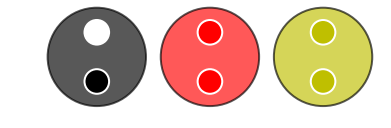
\includegraphics[scale=0.14]{content/optimal/tree_sol/moves/0.png}}
child{node{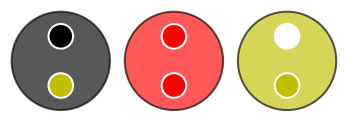
\includegraphics[scale=0.14]{content/optimal/tree_sol/moves/1.png}}
child{node{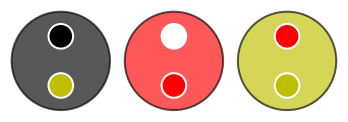
\includegraphics[scale=0.14]{content/optimal/tree_sol/moves/3.png}}}
child{node{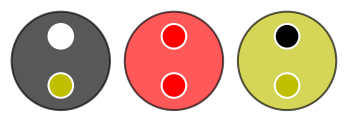
\includegraphics[scale=0.14]{content/optimal/tree_sol/moves/4.png}}}}
child{node{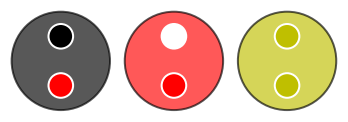
\includegraphics[scale=0.14]{content/optimal/tree_sol/moves/2.png}}
child{node{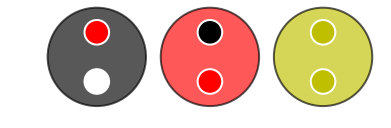
\includegraphics[scale=0.14]{content/optimal/tree_sol/moves/5.png}}}
child{node{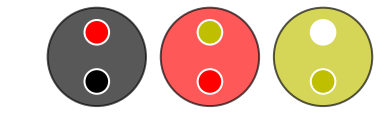
\includegraphics[scale=0.14]{content/optimal/tree_sol/moves/6.png}}}};
    \end{tikzpicture}
\end{center}



Avec un mouvement de plus, nous avons l'arbre ci-dessous (qui n'est pas symétrique : voir en bas à gauche).


\begin{center}
    \begin{tikzpicture}[
    rotate=0,
    level distance=1.5cm,
        level 1/.style={sibling distance=8.5cm},
        level 2/.style={sibling distance=4.75cm},
        level 3/.style={sibling distance=2cm},
    ]
    \node{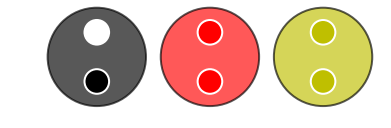
\includegraphics[scale=0.12]{content/optimal/tree_sol/moves/0.png}}
child{node{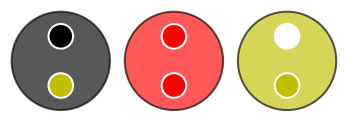
\includegraphics[scale=0.12]{content/optimal/tree_sol/moves/1.png}}
child{node{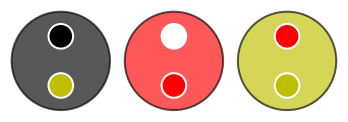
\includegraphics[scale=0.12]{content/optimal/tree_sol/moves/3.png}}
child{node{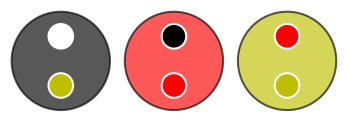
\includegraphics[scale=0.12]{content/optimal/tree_sol/moves/7.png}}}
child{node{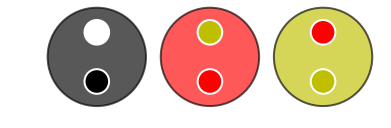
\includegraphics[scale=0.12]{content/optimal/tree_sol/moves/8.png}}}
child{node{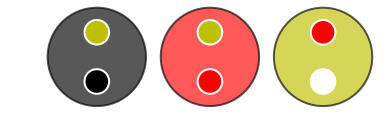
\includegraphics[scale=0.12]{content/optimal/tree_sol/moves/9.png}}}}
child{node{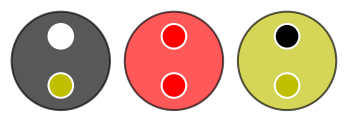
\includegraphics[scale=0.12]{content/optimal/tree_sol/moves/4.png}}
child{node{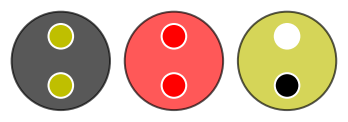
\includegraphics[scale=0.12]{content/optimal/tree_sol/moves/10.png}}}
child{node{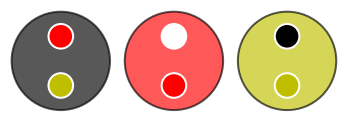
\includegraphics[scale=0.12]{content/optimal/tree_sol/moves/11.png}}}}}
child{node{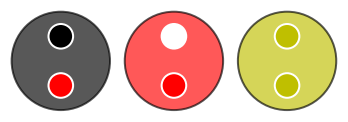
\includegraphics[scale=0.12]{content/optimal/tree_sol/moves/2.png}}
child{node{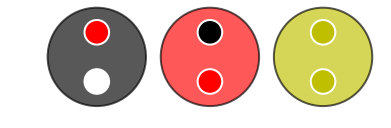
\includegraphics[scale=0.12]{content/optimal/tree_sol/moves/5.png}}
child{node{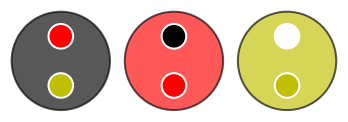
\includegraphics[scale=0.12]{content/optimal/tree_sol/moves/12.png}}}
child{node{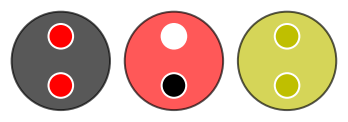
\includegraphics[scale=0.12]{content/optimal/tree_sol/moves/13.png}}}}
child{node{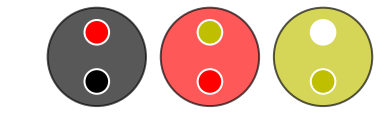
\includegraphics[scale=0.12]{content/optimal/tree_sol/moves/6.png}}
child{node{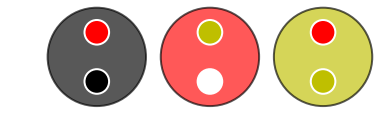
\includegraphics[scale=0.12]{content/optimal/tree_sol/moves/14.png}}}
child{node{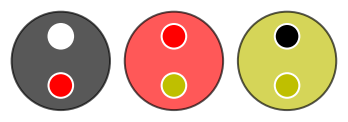
\includegraphics[scale=0.12]{content/optimal/tree_sol/moves/15.png}}}}};
    \end{tikzpicture}
\end{center}



Avec de la patience, ou grâce à un programme, on peut fabriquer l'arbre complet (vous le trouverez en annexe). Notons que pour un jeu à cinq bases, il y a tout de même $11\,010$ configurations (ceci est justifié en annexe), donc représenter l'arbre complet pour 5 bases sur une feuille A3, même avec l'aide d'un programme, ne sera pas possible. 


\medskip

Il est évident que la méthode que nous employons va finir par trouver toutes les configurations tout en nous indiquant leur résolution en faisant le minimum de coups possible. 


\medskip

Notre démarche peut se traduire par l'algorithme ci-dessous où nous utilisons des dictionnaires qui sont des objets associant une valeur à une clé. Par exemple, \verb+mon_dico = {"un": 1, "deux": 2}+ admet pour clés \verb+"un"+ et \verb+"deux"+, et nous notons \verb+mon_dico<"un"> = 1+ la valeur associée à la clé \verb+"un"+.
Nous utilisons aussi $[ \,\, ]$ pour indiquer une liste vide prête à être remplie.


\bigskip

\begin{algo}
	\Data{une configuration quelconque de début de jeu}
	\Result{la solution gagnante (en utilisant le moins de déplacements possible)}
	\vspace{0.4em}
    \Begin{
		\vspace{0.4em}
		$\cal G$ désigne la configuration gagnante.
		\\
		\vspace{0.4em}
		\tcp{"L'arbre" sera construit sous forme d'un dictionnaire.}
		\tcp{\quad \textbullet{} les clés sont les configurations possibles.}
		\tcp{\quad \textbullet{} chaque valeur donne la liste des configurations à suivre pour gagner}
		\tcp{\phantom{\quad \textbullet{}} le plus rapidement possible (lecture de la liste de gauche à droite).}
		$\mathcal{A} \leftarrow \{ \mathcal{G} : [ \,\, ] \}$ 
		\\
		\vspace{0.4em}
		\tcp{Liste stockant les [n]ouvelles [c]onfigurations d'où partir.}
		$NC \leftarrow \big[ \, \mathcal{G} \, \big]$
		\\
		\vspace{0.4em}
		\While{$NC$ n'est pas vide}{
			\vspace{0.4em}
			$NC_{ap} \leftarrow [ \,\, ]$ va stocker les configurations d'où partir durant l'étape d'après.
			\\
			\vspace{0.4em}
			\ForEach{configuration $\mathcal{C}$ dans $NC$}{
				\ForEach{configuration $\mathcal{V}$ obtenue en un seul mouvement depuis $\mathcal{C}$}{
					\If{$\mathcal{V}$ n'est pas une clé de $\cal A$}{
						\vspace{0.4em}
						Ajouter $\mathcal{V}$ à $NC_{ap}$.
						\\
						\vspace{0.4em}
						$COUPS$ : liste obtenue en ajoutant $\mathcal{C}$ à gauche de la liste $\mathcal{A} \big\langle \mathcal{C} \big\rangle$.
						\\
						Ajouter $\mathcal{V}$ à $\mathcal{A}$ avec $\mathcal{A} \big\langle \mathcal{V} \big\rangle = COUPS$.
					}
				}
			}
			\vspace{0.4em}
			$NC \leftarrow NC_{ap}$
		}
		\vspace{0.4em}
		\tcp{Utilisation de l'arbre pour résoudre le jeu.}
		\vspace{0.4em}
		$\mathcal{C}_0$ : la configuration à résoudre.
		\\
		Obtenir successivement les configurations stockées de gauche à droite dans $\mathcal{A} \big\langle \mathcal{C}_0 \big\rangle$.
    }
\end{algo}


\paragraph{Remarque :} \hspace{-1em} l'algorithme présenté dans cette section est facile à programmer mais il devient inutilisable par un humain dès le jeu à quatre bases qui permet d'avoir $480$ configurations différentes (voir l'annexe pour le calcul de cette valeur).
